\documentclass[a4paper,12pt]{extarticle}
\usepackage[table,xcdraw]{xcolor}
\usepackage{pgfplots}
\usepackage[unicode, pdftex]{hyperref}
\usepackage[T2A]{fontenc}
\usepackage[utf8]{inputenc}
\usepackage[english,russian]{babel}
\usepackage{amsmath,amsfonts,amsthm, mathtools}
\usepackage{amssymb}
\usepackage{dsfont}
\usepackage{graphicx}
\graphicspath{{images/}}
\usepackage{wrapfig}
\usepackage{floatrow}
\usepackage{setspace}
\usepackage[headings]{fancyhdr}
\usepackage[margin=10pt,font={small,stretch=0,9},labelfont=bf,labelsep=period,
justification=centerlast]{caption}
\usepackage{array,tabularx,tabulary,booktabs}
\RequirePackage{multirow}
\RequirePackage{multicol}
\RequirePackage{longtable}
\usepackage{indentfirst}
\usepackage{hyperref}
\usepackage{icomma}
\newcommand*{\hm}[1]{#1\nobreak\discretionary{}
	{\hbox{$\mathsurround=0pt #1$}}{}}
\usepackage{soulutf8} 
\usepackage{etoolbox} 
\usepackage{geometry}
\geometry{top=20mm}
\geometry{bottom=20mm}
\geometry{left=20mm}
\geometry{right=20mm}
\DeclareMathOperator{\sgn}{\mathop{sgn}}
\usepackage[OT1]{fontenc}
\usepackage{amsmath}
\usepackage{amsfonts}
\usepackage{amssymb}
\usepackage{wasysym}
\usepackage{wrapfig}
\usepackage{physics}
\usepackage[normalem]{ulem}
\graphicspath{{pictures/}}
\DeclareGraphicsExtensions{.png,.jpg,.jpeg}
\usepackage{indentfirst}
\usepackage[T2A]{fontenc}
\usepackage{subfigure}
\usepackage{fancyhdr}
\usepackage{caption}

\usepackage{tabularx}
\usepackage{floatrow}
\usepackage{multicol}
\usepackage{lastpage}

\pgfplotsset{
  MyStyle1/.style={
    axis lines = middle,
    enlargelimits = true,
    grid=both,
    grid style={line width=.1pt, draw=gray!10},
    major grid style={line width=.2pt,draw=gray!50},
    minor tick num=5,
    enlargelimits=0.05,
    ticklabel style={font=\tiny,fill=white},
    xlabel style={at={(ticklabel* cs:1)},anchor=north west},
    ylabel style={at={(ticklabel* cs:1)},anchor=south east},
  }
}
\def\Slope{1.5}
\def\Intercept{-20}


% Настройка отчёркиваний и нумерации
\usepackage{fancyhdr}
\pagestyle{fancy}
\fancyhf{}

\fancyhead[L]{\nouppercase{\leftmark\hfill}}
\fancyfoot[RO, RE]{Страница \thepage \ из \pageref{LastPage}}
\renewcommand{\headrulewidth}{0.5pt}
\renewcommand{\footrulewidth}{0.5pt}

\usepackage{titlesec}
\titlelabel{\thetitle.\quad}

\pgfplotsset{compat=1.18}
\begin{document}

\thispagestyle{empty}
\begin{center}
	\textit{Федеральное государственное автономное образовательное\\ учреждение высшего образования }
	
	\vspace{0.5ex}
	
	\textbf{«Московский физико-технический институт\\ (национальный исследовательский университет)»}
\end{center}

\vspace{10ex}
\begin{figure}[!h]
  \begin{center}
    
\includegraphics[width = 0.8\textwidth]{MIPT.png}
  \end{center}
\end{figure}

\begin{center}
	
	\textbf{Лабораторная работа №5.10.1}
	
	\vspace{1ex}
	
	по курсу общей физики
	
	на тему:
	
	\textbf{\textit{<<Электронный парамагнитный резонанс (ЭПР)>>}}
	
	\vspace{20ex}
	
	\begin{flushright}
		\noindent
		\textit{Работу выполнил:}\\  
		\textit{Легких Никита \\(группа Б05-301)}
	\end{flushright}
	\vfill
	Долгопрудный \\ \today
	\setcounter{page}{1}
\end{center}
\newpage

% Конец шаблона
\newpage

\textbf{Цель работы:} Исследовать электронный парамагнитный резонанс в молекуле дифенилпикрилгидразила $C_{18}H_{12}N_50_6$, определить $g$-фактор электрона.  \\ \\
\section*{Теоретическая справка} 

В методе ЭПР изучается резонансное поглощение переменного электромагнитного поля в образце в зависимости от контролируемых экспериментатором внешних условий: постоянного магнитного поля, частоты колебаний переменного поля, температуры и так далее.
 
\begin{figure}[h]
\begin{center}

\includegraphics[width = 0.7\textwidth]{pics/1.jpg}
\caption{Схема резонансного поглощения электромагнитного излучения для изолированного спина $S=1/2$. (a) Зеемановское расщепление спинового уровня в магнитном поле. (б) Переход между подуровнями «снизу-вверх» с поглощением фотона резонансной частоты $h\nu=g\mu B$  . (в) Переход между подуровнями «сверху-вниз» с излучением дополнительного фотона резонансной частоты.}
\end{center}
\end{figure}

Простейшей моделью рассмотрения ЭПР является система из невзаимодействующих частиц со спином $S = 1/2$, помещенная во внешнее магнитное поле. В отсутствии поля проекции спинов на ось совпадают, как и энергии. При подаче магнитного поля и эффекта Зеемана энергии с различными направлениями спина начинают различаться. А если мы в систему направим поток фотонов с этой энергией разности этих энергий, то станут возможны индуцированные переходы межу этими состояниями. 

Для наблюдения этого поглощения необходимо резонансное совпадение частоты излучения с
зеемановским расщеплением спиновых подуровней.

Измеряемой в эксперименте величиной является поглощаемая в образце мощность
излучения. Для увеличения точности измерения желательно увеличить эту поглощаемую
мощность.
\newpage
Поглощение переменного магнитного поля в образце описывается мнимой частью магнитной
восприимчивости

\begin{equation}
P_{\text{погл}} = \frac{1}{2}\omega b^2 \chi''(\omega, B)
\end{equation}
где $\omega$ --- частота переменного поля, $b$ --- амплитуда однородного по малому образцу переменного поля, $B$ --- постоянное магнитное поле, $\chi''$ ---  мнимая часть высокочастотной магнитной восприимчивости. Магнитная восприимчивость связывает намагниченность $\vec{m}$ с подмагничивающим магнитным полем $\vec{b} : \vec{m} =\chi \vec{b}$. Комплексное представление восприимчивости имеет смысл для описания отклика на переменное поле $\vec{b}=\vec{b}_0 \cdot e^{-i \omega t}$. Тогда $\vec{m} =\chi \vec{b} = (\chi' + i \chi'')\vec{b}_0 e^{-i \omega t}=\chi' \vec{b}_0 e^{-i \omega t} + \chi'' \vec{b}_0 e^{-i \omega t + \frac{pi}{2}}$. Таким образом, действительная часть высокочастотной восприимчивости описывает вклад в
намагниченность, находящийся в фазе с подмагничивающим полем, а мнимая часть — вклад, сдвинутый
относительно подмагничивающего поля по фазе на $\frac{\pi}{2}$. Естественно, при $\omega=0$ мнимая часть восприимчивости $\chi'' = 0$. Сдвиг по фазе отклика (намагниченности) относительно вынуждающей силы
(переменного поля) связан с потерями энергии, поэтому мнимая часть восприимчивости является мерой
диссипации энергии в системе.

{\large\textbf{\subsection*{Физические причины возникновения резонансного поглощения в
парамагнетике}}}
Простейшей системой для изучения методом ЭПР является парамагнетик — система слабо
взаимодействующих атомов, ионов или молекул, обладающих собственным магнитным
моментом. Пренебрегая взаимодействием, можно рассмотреть поведение магнитного диполя
в постоянном и переменном магнитном поле. 

В «классическом» подходе рассматривается прецессия магнитного момента во внешнем поле
при отклонении магнитного момента от равновесия. Классический магнитный диполь
стремится выровняться вдоль силовых линий магнитного поля, при отклонении от
равновесия возникает возвращающий механический момент $\vec{T}=\vec{M}\times \vec{B}$ . Так как
магнитный и механический момент иона связаны друг с другом гиромагнитным отношением
$\gamma$ как $\vec{M} =\gamma \vec{I}$ , где $\vec{I}$ - это полный момент импульса, то с учётом уравнения динамики $\frac{d\vec{I}}{dt} = \vec{T}$ получим уравнение прецессии магнитного момента $\frac{d\vec{M}}{dt} = \gamma \vec{M}\times \vec{B}$. Аналогично
с известной задачей о прецессии гироскопа можно заметить, что при отклонении магнитного
момента от направления магнитного поля возникает незатухающая прецессия вокруг
направления поля с угловой скоростью $\vec{\Omega}= - \gamma \vec{B}$ , частота этой прецессии $\Omega_L=\gamma B$
называется ларморовской. При совпадении частоты переменного поля с ларморовской
частотой возможно возникновение резонансного поглощения.

Расщепление терма свободного иона (или молекулы) определяется спектроскопическим
фактором Ланде ($g$-фактором Ланде): $E(m_J)=g\mu_B B m_J$.

\begin{equation}
g_{\text{эфф}} = \frac{h \nu}{\mu_B B}
\end{equation}
\newpage
\section*{Установка}

В данной работе мы исследуем данную молекулу

\begin{figure}[h]
\begin{center}

\includegraphics[width = 0.4\textwidth]{pics/2.jpg}
\caption{Химическая структура молекулы}
\end{center}
\end{figure}

Схема установки выглядит следующим образом:

\begin{wrapfigure}{r}{0.5\textwidth}
  \begin{center}
    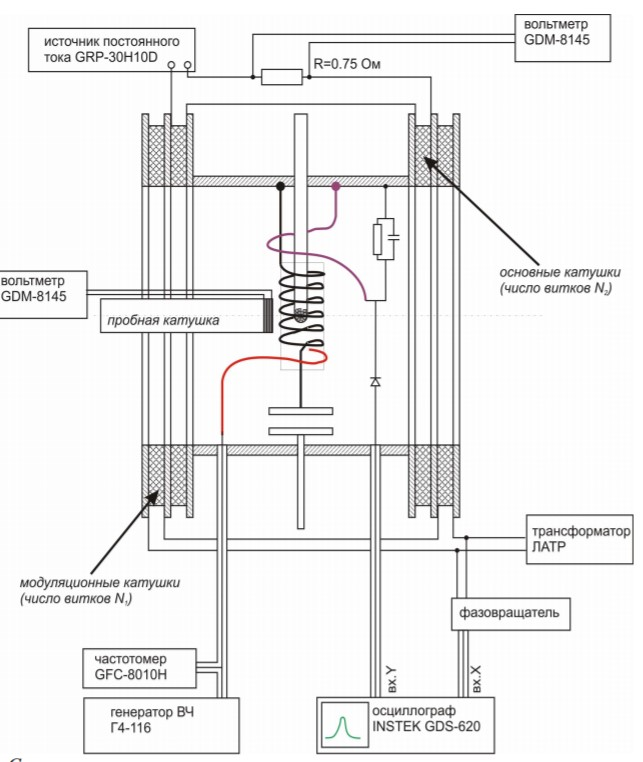
\includegraphics[width = 1\textwidth]{pics/3.jpg}
  \end{center}
  \caption{Схема установки}
\end{wrapfigure}

Схема установки представлена на Рис. 3. Образец (порошок ДФПГ) в стеклянной ампуле помещается внутрь катушки индуктивности, входящей в состав колебательного контура. Входящий в состав контура конденсатор состоит из двух пластин, разделённых воздушным зазором, одна из пластин может перемещаться поворотом штока. Колебания в контуре возбуждаются антенной, соединённой с генератором высокой частоты (ВЧ) Г4-116. Амплитуда колебаний поля в катушке индуктивности измеряется по наводимой в петле связи ЭДС индукции. Высокочастотные колебания ЭДС индукции в приёмном кон-
туре детектируются диодом, измеряемая при помощи осциллографа низкочастотная огибающая этого сигнала пропорциональна квадрату амплитуды колебаний поля в катушке.

Постоянное магнитное поле создаётся пропусканием тока от источника постоянного тока через основные катушки. При этом при помощи вольтметра измеряется падение напряжения на резисторе в цепи основных катушек. Переменное поле небольшой амплитуды создаётся подачей на модуляционные катушки напряжения с регулируемого трансформатора ЛАТР. Для измерения амплитуды колебаний переменного поля используется пробная катушка известной геометрии, подключённая к вольтметру. Пусть поток через неё $\Phi_{\text{проб}},$ тогда ЭДС индукции
$$
\mathcal{E}=-\frac{d \Phi_{\text{проб}}}{d t}
$$
Если $I_{\text{осн}}-$ ток через основную катушку, а $M-$ взаимная индуктивность основной и пробной катушек, то
$$
\Phi_{\text{проб}}=M I_{\text{осн}}
$$
Тогда амплитудное значение ЭДС индукции
$$
\mathcal{E}_{\text {aмп }}=-\frac{d M I_{\text {осн }}}{d t}=M \omega I_{\text {aмп }}
$$

Тогда, зная, что
$$
\Phi_{\text{проб}}=B_{0} N_{\text{проб}} \frac{\pi d_{\text{проб}}^{2}}{4}=\frac{M U_{R}}{R}=\frac{k U}{\omega}
$$
где $U-$ напряжение на $R$ в резонансе, получим
$$
B_{0}=\frac{4 k U}{\pi \omega d_{\text{проб}}^{2} N_{\text{проб}}}
$$
Характеристики катушек: пробная катушка $N_{\text {проб }}=45, d_{\text {проб }}=14.5 \pm 0.1$ мм, основная катушка $N_{\text {осн }}=4500, d_{\text {осн }}=0.29 \pm 0.01$ м, модулирующая катушка $N_{\text {мод }}=1500, d_{\text {мод }}=$ $0.29 \pm 0.01$ м.


%%%%%%%%%%%%%%%%%%%%%%%%%%%%%%

\section*{Ход работы}
\subsection*{Настройка высокочастотного генератора}
Генератор настраиваем на частоту колебательного контура: в режиме амплитудной модуляции $10 \%$ устанавливаем подстройкой частоты генератора добиваемся максимальной амплитуды сигнала на экране осциллографа. Частоту определяем по шкале генератора, $f_{0}=139.9 \pm 0.1$ МГц (погрешность всех измерений частот - цена деления грубой шкалы $\sigma_{f}=0.1$ МГц $) .$ 


% Также для вычисления добротности расстроим частоту до достижения сигналом половины от максимального значения. Тогда, если $f_{\pm \frac{1}{2}}$ - значения частот при достижении половинного сигнала при расстройке генератора в сторону больших и маленьких частот, то добротность
% $$
% Q=\frac{f_{0}}{f_{+\frac{1}{2}}-f_{-\frac{1}{2}}}
% $$
% $$
% Q=100 \pm 20
% $$
% где погрешность рассчитана по формуле
% $$
% \sigma_{Q}=\sigma_{f} \sqrt{\left(\frac{\partial Q}{\partial f_{0}}\right)^{2}+\left(\frac{\partial Q}{\partial f_{+\frac{1}{2}}}\right)^{2}+\left(\frac{\partial Q}{\partial f_{-\frac{1}{2}}}\right)^{2}}
% $$



\subsection*{Наблюдение сигнала резонансного поглощения}
Подключим основные катушки к источнику постоянного тока, а модуляционные катушки к трансформатору ЛАТР. ВЧ-генератор переведём в режим непрерывной генерации, на канале осциллографа, подключённому к детектору, установим максимальную чувствительность. Подадим на модуляционные катушки напряжение $\sim 21$ В, и, плавно увеличивая постоянное напряжение на основных катушках, добиваемся возникновения на экране резонанстного поглощения. Добъёмся того, чтобы наблюдаемые пики были максимального размера. Зафиксируем напряжение $U=40.0 \pm 0.5$ мВ напряжение на резисторе $R$.
\subsection*{Определение $g$-фактора и определение ширины линии}
Для определения ширины линии резонансного поглощения удобно подать на Х-канал осциллографа напряжение, прикладываемое к модуляционным катушкам и наблюдать сигнал в ХY-режиме. Фактически при этом на экране наблюдается зависимость поглощения в образце от приложенного переменного поля. Наблюдаемая картина симметрична относительно средней вертикальной оси. Из-за набегающей в электрической схеме расфазировки напряжений на экране наблюдаются два пика, соответствующие прохождению резонансного поглощения на растущем и падающем полупериодах модулирующего напряжения, поэтому пики совмещаем подстройкой фазовращателя (что было сделано еще в прошлом пункте, для простоты определения данных). Для определения ширины линии ЭПР определим по экрану осциллографа полный размах модулирующего поля $A_{\text {полн }} = 7.6\pm0.2$ и полную ширину кривой резонансного поглощения на полувысоте $A_{1 / 2} = 0.6\pm0.2$ (погрешность берем как цену деления). 

\begin{figure}[h]
\begin{center}
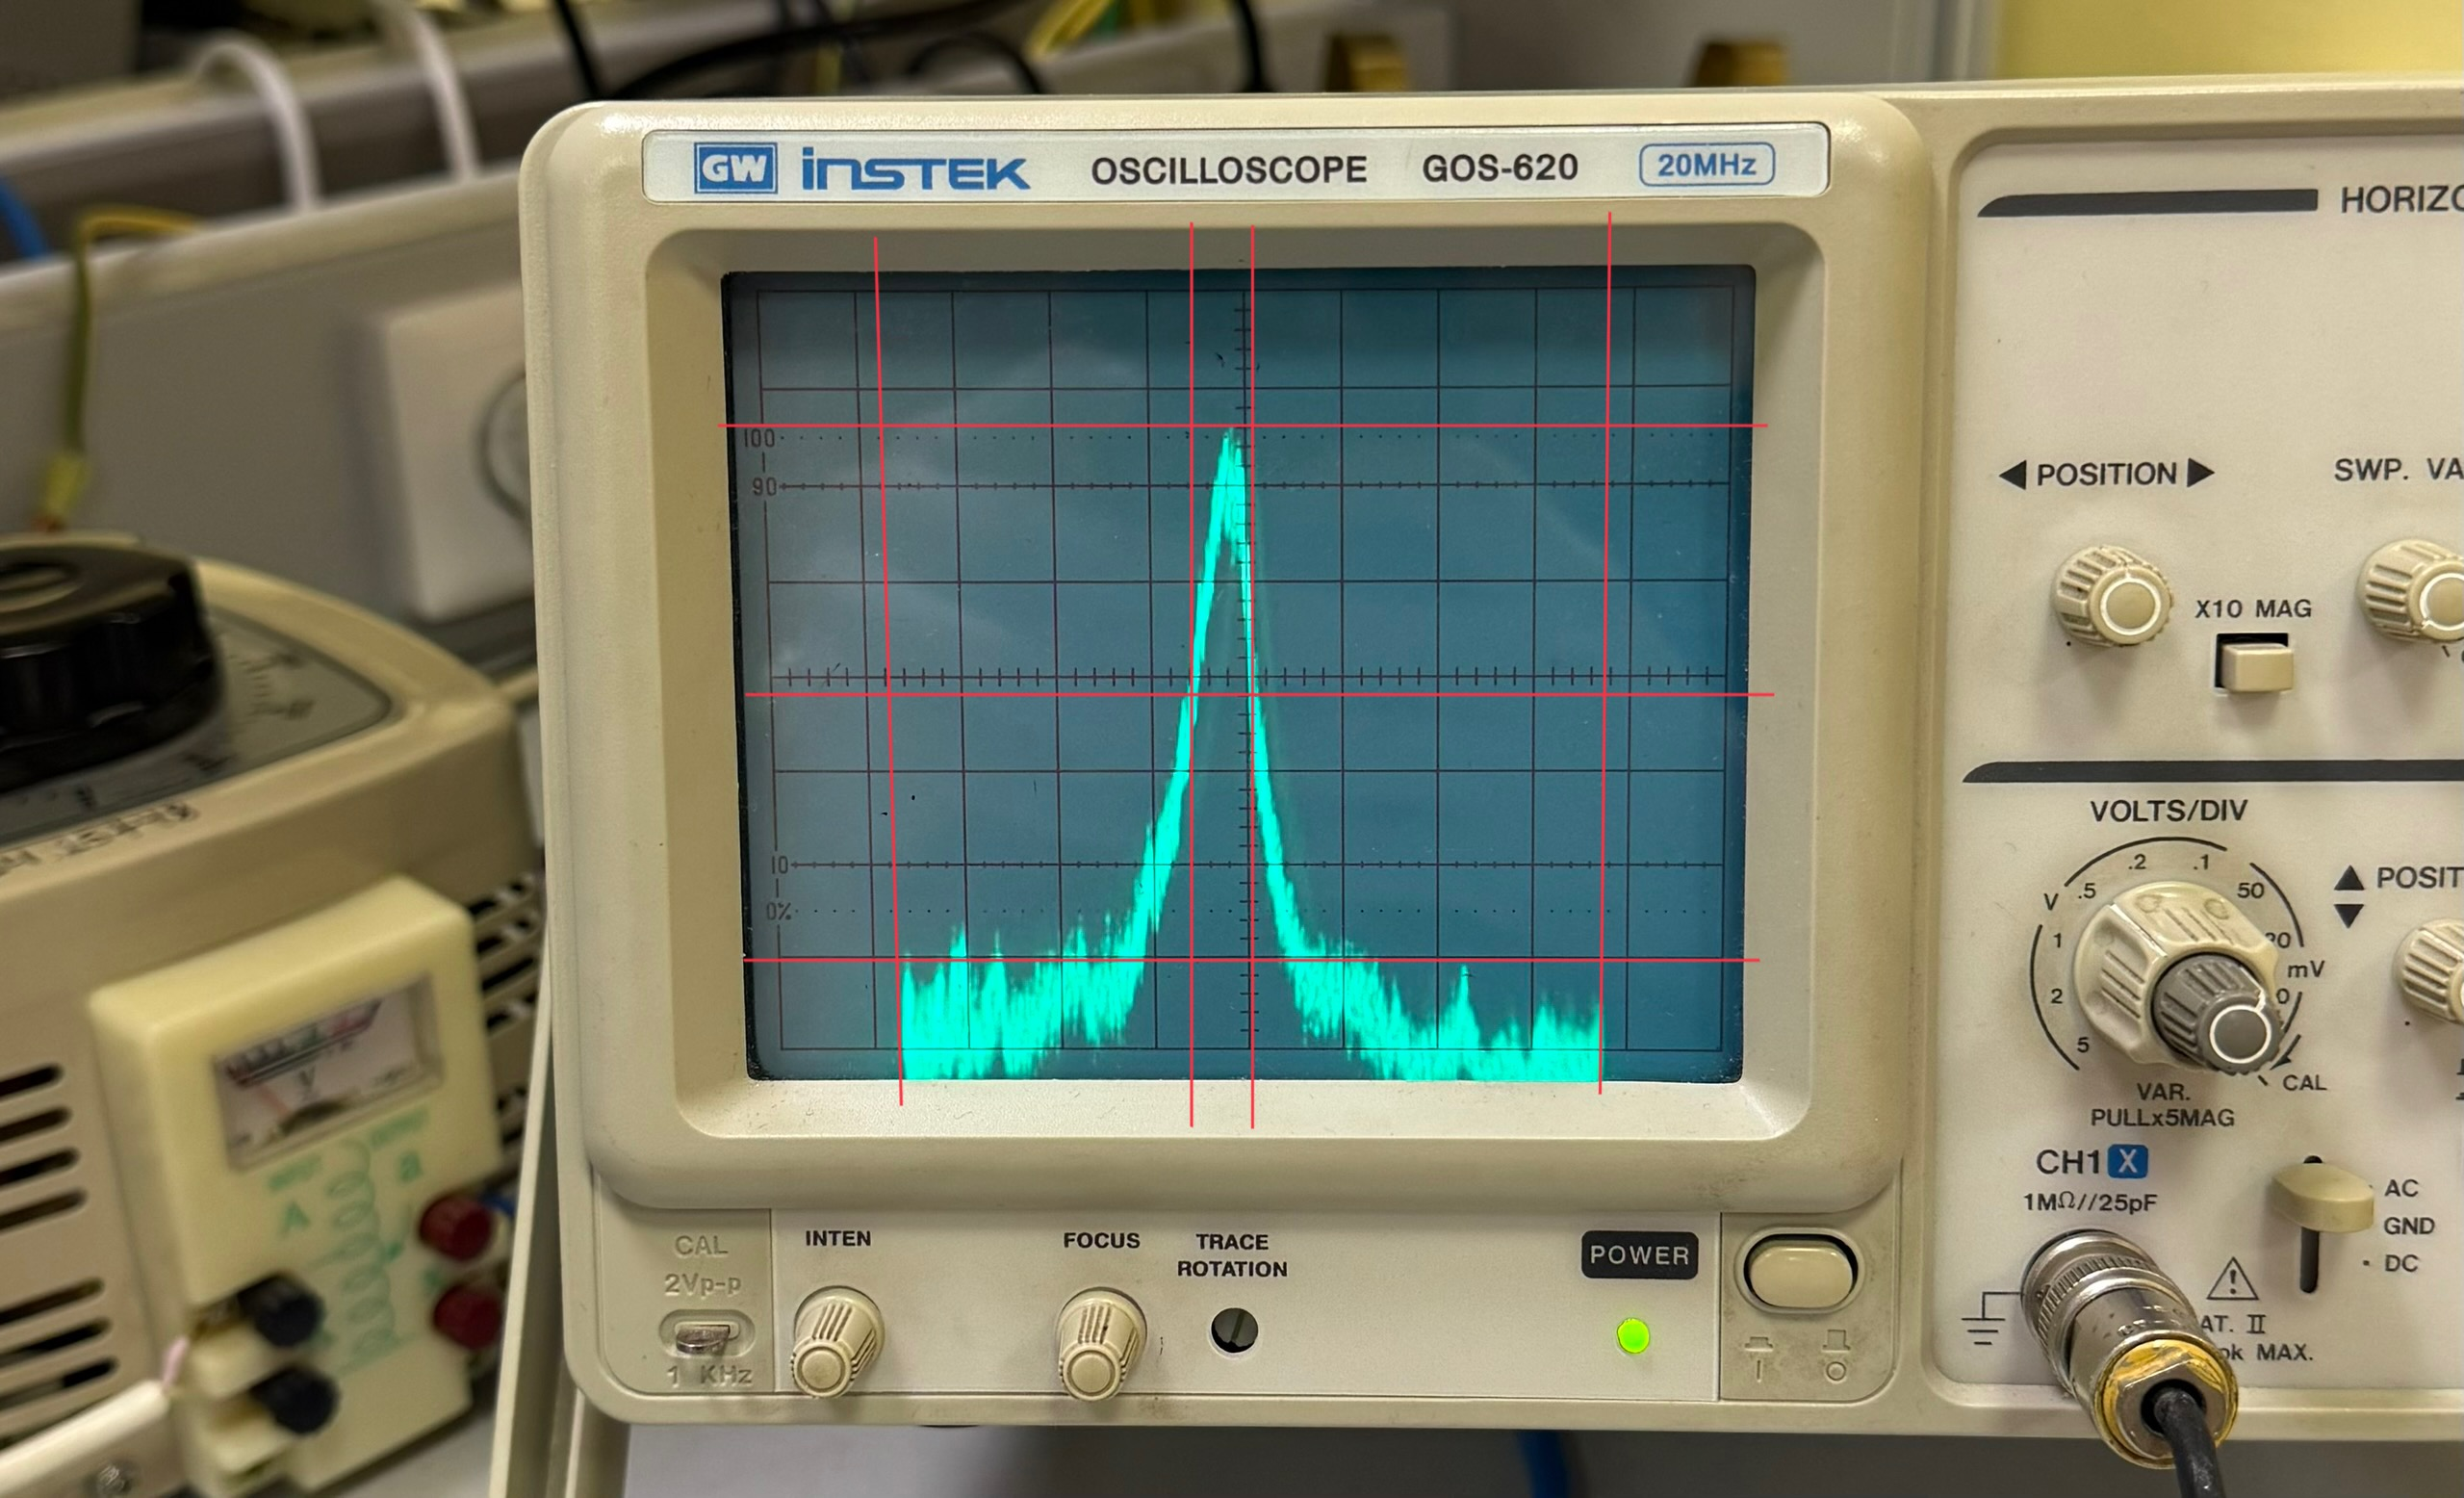
\includegraphics[width = 0.7\textwidth]{pics/4.jpeg}
\caption{Видимая картинка на экране осциллографа}
\end{center}
\end{figure}

Для измерения действующего поля, переключаем катушки на переменное поле и добиваемся на катушках такого же действующего напряжения как было до этого постоянное. И смотрим на значение напряжения на пробной катушке $\mathcal{E} = 1.41$ мВ.

Тогда амплитуда модулирующего поля
$$
B_{\text {мод }}=\frac{2 \mathcal{E}}{\pi^{2} d_{\text {проб }}^{2} N_{\text {проб }} \nu}=6.0 \pm 0.2 \text { мТл }
$$
где погрешность рассчитана по формуле
$$
\sigma_{B_{\text {мод }}}=\sqrt{\left(\frac{\partial B_{\text {Мод }}}{\partial \mathcal{E}}\right)^{2} \sigma_{\mathcal{E}}^{2}+\left(\frac{\partial B_{\text {Мод }}}{\partial d_{\text {проб }}}\right)^{2} \sigma_{d_{\text {проб }}}^{2}}
$$
где $\nu=50$ Гц - частота модулирующего напряжения. Полуширину на полувысоте линии резонансного поглощения посчитаем по формуле
$$
\Delta B=\frac{A_{1 / 2}}{A_{\text {полн }}} B_{\text {мод }}=0.67 \pm 0.01 \text { мТл }
$$
где погрешность рассчитана по формуле
$$
\sigma_{\Delta B}=\sqrt{\left(\frac{\partial \Delta B}{\partial A_{\text {полн }}}\right)^{2} \sigma_{A_{\text {полн }}}^{2}+\left(\frac{\partial \Delta B}{\partial A_{1 / 2}}\right)^{2} \sigma_{A_{1 / 2}}^{2}+\left(\frac{\partial \Delta B}{\partial B_{\text {мод }}}\right)^{2} \sigma_{B_{\text {мод }}}^{2}}
$$



Для определения поля резонансного поглошения найдём связь между падением напряжения на резисторе в цепи основной катушки и магнитным полем. Для этого подадим в основные катушки переменный ток и измеряем при помощи пробной катушки ЭДС индукции. Переключим основные катушки на ЛАТР, переведём вольтметр, измеряющий падение напряжения на резисторе $V_{R}$ в цепи основных катушек, в режим измерений на переменном токе, установите ток через катушки, близкий к значению тока при наблюдении резонансного поглощения, измерим в этих условиях ЭДС индукции в пробных катушках. Для контроля однородности поля вносим катушку в центр магнита с передней $\left(V_{\text {перед }}\right)$ и задней $\left(V_{\text {зад }}\right)$ стороны установки. Для повышения точности калибровочные измерения проведём при нескольких значениях тока через катушку.

$$
B_{0}=\frac{4 U}{\pi \omega d_{\mathrm{Irpo} 0}^{2} N_{\text{проб}}}=8.5 \pm 0.2 \text{мТл}
$$
а погрешность рассчитывалась по формуле:
$$
\sigma_{B_{0}}=\sqrt{\left(\frac{\partial B_{0}}{\partial k}\right)^{2} \sigma_{k}^{2}+\left(\frac{\partial B_{0}}{\partial U_{R}}\right)^{2} \sigma_{U_{R}}^{2}+\left(\frac{\partial B_{0}}{\partial d_{\text {проб }}}\right)^{2} \sigma_{d_{\text {проб }}}^{2}}
$$
Тогда $g$ -фактор электрона будет по формуле (1) равен
$$
g=\frac{h f_{0}}{\mu_{B} B_{0}}=1.81 \pm 0.12
$$
погрешность считалась по формуле
$$
\sigma_{g}=\sqrt{\left(\frac{\partial g}{\partial f_{0}}\right)^{2} \sigma_{f_{0}}^{2}+\left(\frac{\partial g}{\partial B_{0}}\right)^{2} \sigma_{B_{0}}^{2}}
$$
Истинное значение $g$ -фактора электрона $g=2.0036$ (значение взято из Глазков В.Н. Работа 10.1: Электронный парамагнитный резонанс. Дополнительное описание работы. MФTИ, 2016 .) почти лежит в пределах доверительного интервала.
\section*{Вывод}
В данной работе был исследован ЭПР в молекуле ДФПГ, определяется $g$ -фактор электрона $g=1.81 \pm 0.12,$ а также измерена ширина линий ЭПР $\Delta B=0.67 \pm 0.01$ мТл.

\begin{thebibliography}{9}
\bibitem{laba1} 
Глазков В.Н. 
\textit{Работа 10.1: Электронный парамагнитный резонанс.
Дополнительное описание работы}. 
МФТИ, 2016.
\bibitem{laba2} 
Глазков В.Н. 
\textit{Инструкции по выполнению работы 10.1}. 
МФТИ, 2016.
\end{thebibliography}

\end{document}